\documentclass{standalone}
\usepackage{tikz}
\usetikzlibrary{patterns, positioning}


\begin{document}
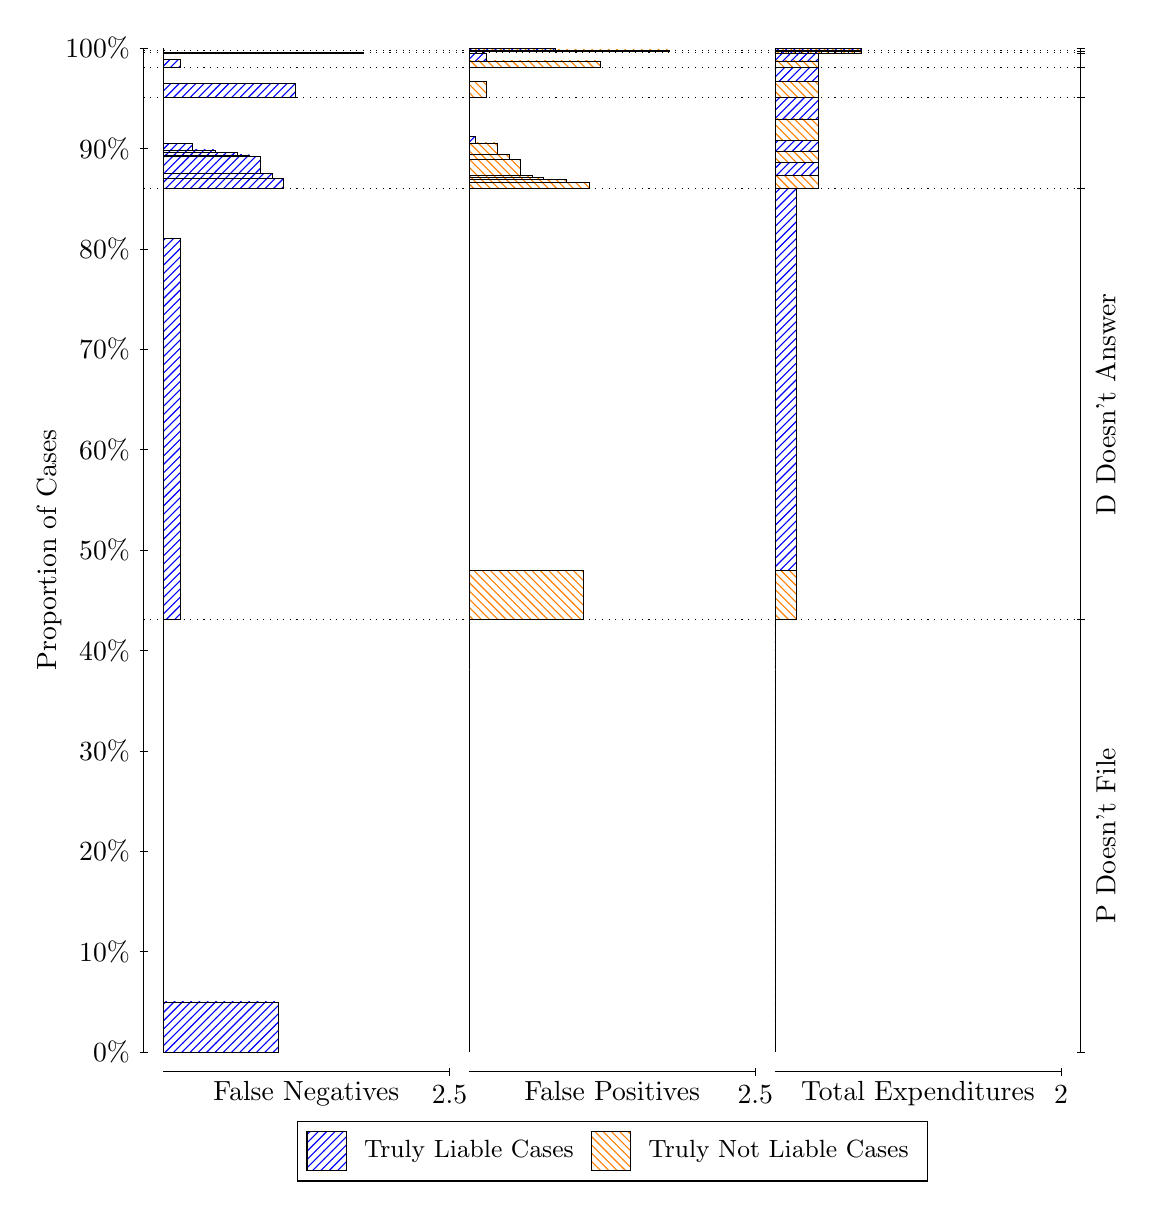
\begin{tikzpicture}
\draw[black, very thin] (1.5,1.75) -- (1.5,14.5);
\node[rotate=90, text=black, anchor=center] at (0.3, 8.125) {Proportion of Cases};
\draw[black, very thin] (1.45,1.75) -- (1.55,1.75);
\node[text=black, anchor=east] at (1.45, 1.75) {0\%};
\draw[black, very thin] (1.45,3.025) -- (1.55,3.025);
\node[text=black, anchor=east] at (1.45, 3.025) {10\%};
\draw[black, very thin] (1.45,4.3) -- (1.55,4.3);
\node[text=black, anchor=east] at (1.45, 4.3) {20\%};
\draw[black, very thin] (1.45,5.575) -- (1.55,5.575);
\node[text=black, anchor=east] at (1.45, 5.575) {30\%};
\draw[black, very thin] (1.45,6.85) -- (1.55,6.85);
\node[text=black, anchor=east] at (1.45, 6.85) {40\%};
\draw[black, very thin] (1.45,8.125) -- (1.55,8.125);
\node[text=black, anchor=east] at (1.45, 8.125) {50\%};
\draw[black, very thin] (1.45,9.4) -- (1.55,9.4);
\node[text=black, anchor=east] at (1.45, 9.4) {60\%};
\draw[black, very thin] (1.45,10.675) -- (1.55,10.675);
\node[text=black, anchor=east] at (1.45, 10.675) {70\%};
\draw[black, very thin] (1.45,11.95) -- (1.55,11.95);
\node[text=black, anchor=east] at (1.45, 11.95) {80\%};
\draw[black, very thin] (1.45,13.225) -- (1.55,13.225);
\node[text=black, anchor=east] at (1.45, 13.225) {90\%};
\draw[black, very thin] (1.45,14.5) -- (1.55,14.5);
\node[text=black, anchor=east] at (1.45, 14.5) {100\%};

\draw[black, very thin] (13.4,1.75) -- (13.4,14.5);
\draw[black, very thin] (13.35,1.75) -- (13.45,1.75);
\node[anchor=west] at (13.35, 1.75) {};
\draw[black, very thin] (13.35,7.2412) -- (13.45,7.2412);
\node[anchor=west] at (13.35, 7.2412) {};
\draw[black, very thin] (13.35,12.714) -- (13.45,12.714);
\node[anchor=west] at (13.35, 12.714) {};
\draw[black, very thin] (13.35,13.872) -- (13.45,13.872);
\node[anchor=west] at (13.35, 13.872) {};
\draw[black, very thin] (13.35,14.254) -- (13.45,14.254);
\node[anchor=west] at (13.35, 14.254) {};
\draw[black, very thin] (13.35,14.438) -- (13.45,14.438);
\node[anchor=west] at (13.35, 14.438) {};
\draw[black, very thin] (13.35,14.465) -- (13.45,14.465);
\node[anchor=west] at (13.35, 14.465) {};
\draw[black, very thin] (13.35,14.5) -- (13.45,14.5);
\node[anchor=west] at (13.35, 14.5) {};

\draw[black, very thin, pattern color=blue, pattern=north east lines] (1.75,1.75) rectangle (3.2033,2.386);
\draw[black, very thin, pattern color=orange, pattern=north west lines] (1.75,2.386) rectangle (1.75,7.2412);
\draw[black, very thin, pattern color=blue, pattern=north east lines] (1.75,7.2412) rectangle (1.968,12.087);
\draw[black, very thin, pattern color=orange, pattern=north west lines] (1.75,12.087) rectangle (1.75,12.714);
\draw[black, very thin, pattern color=blue, pattern=north east lines] (1.75,12.714) rectangle (3.276,12.848);
\draw[black, very thin, pattern color=blue, pattern=north east lines] (1.75,12.848) rectangle (3.1307,12.91);
\draw[black, very thin, pattern color=blue, pattern=north east lines] (1.75,12.91) rectangle (2.9853,13.12);
\draw[black, very thin, pattern color=blue, pattern=north east lines] (1.75,13.12) rectangle (2.84,13.143);
\draw[black, very thin, pattern color=blue, pattern=north east lines] (1.75,13.143) rectangle (2.6947,13.172);
\draw[black, very thin, pattern color=blue, pattern=north east lines] (1.75,13.172) rectangle (2.404,13.206);
\draw[black, very thin, pattern color=blue, pattern=north east lines] (1.75,13.206) rectangle (2.1133,13.291);
\draw[black, very thin, pattern color=orange, pattern=north west lines] (1.75,13.291) rectangle (1.75,13.872);
\draw[black, very thin, pattern color=blue, pattern=north east lines] (1.75,13.872) rectangle (3.4213,14.054);
\draw[black, very thin, pattern color=orange, pattern=north west lines] (1.75,14.054) rectangle (1.75,14.254);
\draw[black, very thin, pattern color=blue, pattern=north east lines] (1.75,14.254) rectangle (1.968,14.355);
\draw[black, very thin, pattern color=orange, pattern=north west lines] (1.75,14.355) rectangle (1.75,14.438);
\draw[black, very thin, pattern color=blue, pattern=north east lines] (1.75,14.438) rectangle (4.2933,14.449);
\draw[black, very thin, pattern color=orange, pattern=north west lines] (1.75,14.449) rectangle (1.75,14.465);
\draw[black, very thin, pattern color=orange, pattern=north west lines] (1.75,14.465) rectangle (1.75,14.477);
\draw[black, very thin, pattern color=blue, pattern=north east lines] (1.75,14.477) rectangle (1.75,14.5);
\draw[black, very thin, pattern color=orange, pattern=north west lines] (5.6333,1.75) rectangle (5.6333,6.6052);
\draw[black, very thin, pattern color=blue, pattern=north east lines] (5.6333,6.6052) rectangle (5.6333,7.2412);
\draw[black, very thin, pattern color=orange, pattern=north west lines] (5.6333,7.2412) rectangle (7.0867,7.8678);
\draw[black, very thin, pattern color=blue, pattern=north east lines] (5.6333,7.8678) rectangle (5.6333,12.714);
\draw[black, very thin, pattern color=orange, pattern=north west lines] (5.6333,12.714) rectangle (7.1593,12.795);
\draw[black, very thin, pattern color=orange, pattern=north west lines] (5.6333,12.795) rectangle (6.8687,12.829);
\draw[black, very thin, pattern color=orange, pattern=north west lines] (5.6333,12.829) rectangle (6.578,12.858);
\draw[black, very thin, pattern color=orange, pattern=north west lines] (5.6333,12.858) rectangle (6.4327,12.88);
\draw[black, very thin, pattern color=orange, pattern=north west lines] (5.6333,12.88) rectangle (6.2873,13.09);
\draw[black, very thin, pattern color=orange, pattern=north west lines] (5.6333,13.09) rectangle (6.142,13.153);
\draw[black, very thin, pattern color=orange, pattern=north west lines] (5.6333,13.153) rectangle (5.9967,13.295);
\draw[black, very thin, pattern color=blue, pattern=north east lines] (5.6333,13.295) rectangle (5.706,13.381);
\draw[black, very thin, pattern color=blue, pattern=north east lines] (5.6333,13.381) rectangle (5.6333,13.872);
\draw[black, very thin, pattern color=orange, pattern=north west lines] (5.6333,13.872) rectangle (5.8513,14.073);
\draw[black, very thin, pattern color=blue, pattern=north east lines] (5.6333,14.073) rectangle (5.6333,14.254);
\draw[black, very thin, pattern color=orange, pattern=north west lines] (5.6333,14.254) rectangle (7.3047,14.337);
\draw[black, very thin, pattern color=blue, pattern=north east lines] (5.6333,14.337) rectangle (5.8513,14.438);
\draw[black, very thin, pattern color=orange, pattern=north west lines] (5.6333,14.438) rectangle (5.6333,14.454);
\draw[black, very thin, pattern color=blue, pattern=north east lines] (5.6333,14.454) rectangle (5.6333,14.465);
\draw[black, very thin, pattern color=orange, pattern=north west lines] (5.6333,14.465) rectangle (8.1767,14.477);
\draw[black, very thin, pattern color=blue, pattern=north east lines] (5.6333,14.477) rectangle (6.7233,14.5);
\draw[black, very thin, pattern color=orange, pattern=north west lines] (9.5167,1.75) rectangle (9.5167,6.6052);
\draw[black, very thin, pattern color=blue, pattern=north east lines] (9.5167,6.6052) rectangle (9.5167,7.2412);
\draw[black, very thin, pattern color=orange, pattern=north west lines] (9.5167,7.2412) rectangle (9.7892,7.8678);
\draw[black, very thin, pattern color=blue, pattern=north east lines] (9.5167,7.8678) rectangle (9.7892,12.714);
\draw[black, very thin, pattern color=orange, pattern=north west lines] (9.5167,12.714) rectangle (10.062,12.88);
\draw[black, very thin, pattern color=blue, pattern=north east lines] (9.5167,12.88) rectangle (10.062,13.051);
\draw[black, very thin, pattern color=orange, pattern=north west lines] (9.5167,13.051) rectangle (10.062,13.194);
\draw[black, very thin, pattern color=blue, pattern=north east lines] (9.5167,13.194) rectangle (10.062,13.328);
\draw[black, very thin, pattern color=orange, pattern=north west lines] (9.5167,13.328) rectangle (10.062,13.6);
\draw[black, very thin, pattern color=blue, pattern=north east lines] (9.5167,13.6) rectangle (10.062,13.872);
\draw[black, very thin, pattern color=orange, pattern=north west lines] (9.5167,13.872) rectangle (10.062,14.073);
\draw[black, very thin, pattern color=blue, pattern=north east lines] (9.5167,14.073) rectangle (10.062,14.254);
\draw[black, very thin, pattern color=orange, pattern=north west lines] (9.5167,14.254) rectangle (10.062,14.337);
\draw[black, very thin, pattern color=blue, pattern=north east lines] (9.5167,14.337) rectangle (10.062,14.438);
\draw[black, very thin, pattern color=orange, pattern=north west lines] (9.5167,14.438) rectangle (10.607,14.454);
\draw[black, very thin, pattern color=blue, pattern=north east lines] (9.5167,14.454) rectangle (10.607,14.465);
\draw[black, very thin, pattern color=orange, pattern=north west lines] (9.5167,14.465) rectangle (10.607,14.477);
\draw[black, very thin, pattern color=blue, pattern=north east lines] (9.5167,14.477) rectangle (10.607,14.5);
\draw[black, dotted] (1.5,7.2412) -- (13.4,7.2412);
\draw[black, dotted] (1.5,12.714) -- (13.4,12.714);
\draw[black, dotted] (1.5,13.872) -- (13.4,13.872);
\draw[black, dotted] (1.5,14.254) -- (13.4,14.254);
\draw[black, dotted] (1.5,14.438) -- (13.4,14.438);
\draw[black, dotted] (1.5,14.465) -- (13.4,14.465);
\draw[black, very thin] (1.75,1.5) -- (5.3833,1.5);
\node[text=black, anchor=north] at (3.5667, 1.5) {False Negatives};
\draw[black, very thin] (5.3833,1.45) -- (5.3833,1.55);
\node[text=black, anchor=north] at (5.3833, 1.45) {2.5};

\draw[black, very thin] (5.6333,1.5) -- (9.2667,1.5);
\node[text=black, anchor=north] at (7.45, 1.5) {False Positives};
\draw[black, very thin] (9.2667,1.45) -- (9.2667,1.55);
\node[text=black, anchor=north] at (9.2667, 1.45) {2.5};

\draw[black, very thin] (9.5167,1.5) -- (13.15,1.5);
\node[text=black, anchor=north] at (11.333, 1.5) {Total Expenditures};
\draw[black, very thin] (13.15,1.45) -- (13.15,1.55);
\node[text=black, anchor=north] at (13.15, 1.45) {2};

\node[text=black, centered, rotate=90] at (13.72, 4.4956) {P Doesn't File};
\node[text=black, centered, rotate=90] at (13.72, 9.9774) {D Doesn't Answer};






\draw (7.449999999999999,1.5) node[draw=none] (baseCoordinate) {};
\begin{scope}[align=center]
        \matrix[scale=0.5, draw=black, below=0.5cm of baseCoordinate, nodes={draw}, column sep=0.1cm]{
            \node[rectangle, draw, minimum width=0.5cm, minimum height=0.5cm, pattern color=blue, pattern=north east lines] {}; &
            \node[draw=none, font=\small, text=black] (B) {Truly Liable Cases}; &
            \node[rectangle, draw, minimum width=0.5cm, minimum height=0.5cm, pattern color=orange, pattern=north west lines] {}; &
            \node[draw=none, font=\small, text=black] (B) {Truly Not Liable Cases}; \\
            };
\end{scope}

\end{tikzpicture}
\end{document}